\section{epluszsz.\textless{}ext\textgreater{}}\label{epluszsz.ext}

This file is a result of the zone sizing calculation. Zone Sizing (see Sizing:Zone object) performs a special calculation, using a theoretical ideal zonal system, and determines the zone design heating and cooling flow rates and loads, saving the results in the zone sizing arrays. The file has a similar format to the eplusssz.\textless{}ext\textgreater{} file.

An excerpt (this is a direct copy of the CSV data, so you can copy it to a spreadsheet to view it easier):

Time,SPACE1-1:CHICAGO\_IL\_USA ANNUAL HEATING 99\% DESIGN CONDITIONS DB:Des Heat Load {[}W{]},SPACE1-1:CHICAGO\_IL\_USA ANNUAL COOLING 1\% DESIGN CONDITIONS DB/MCWB:Des Sens Cool Load {[}W{]},SPACE1-1:CHICAGO\_IL\_USA ANNUAL HEATING 99\% DESIGN CONDITIONS DB:Des Heat Mass Flow {[}kg/s{]},SPACE1-1:CHICAGO\_IL\_USA ANNUAL COOLING 1\% DESIGN CONDITIONS DB/MCWB:Des Cool Mass Flow {[}kg/s{]},SPACE2-1:CHICAGO\_IL\_USA ANNUAL HEATING 99\% DESIGN CONDITIONS DB:Des Heat Load {[}W{]},SPACE2-1:CHICAGO\_IL\_USA ANNUAL COOLING 1\% DESIGN CONDITIONS DB/MCWB:Des Sens Cool Load {[}W{]},SPACE2-1:CHICAGO\_IL\_USA ANNUAL HEATING 99\% DESIGN CONDITIONS DB:Des Heat Mass Flow {[}kg/s{]},SPACE2-1:CHICAGO\_IL\_USA ANNUAL COOLING 1\% DESIGN CONDITIONS DB/MCWB:Des Cool Mass Flow {[}kg/s{]},SPACE3-1:CHICAGO\_IL\_USA ANNUAL HEATING 99\% DESIGN CONDITIONS DB:Des Heat Load {[}W{]},SPACE3-1:CHICAGO\_IL\_USA ANNUAL COOLING 1\% DESIGN CONDITIONS DB/MCWB:Des Sens Cool Load {[}W{]},SPACE3-1:CHICAGO\_IL\_USA ANNUAL HEATING 99\% DESIGN CONDITIONS DB:Des Heat Mass Flow {[}kg/s{]},SPACE3-1:CHICAGO\_IL\_USA ANNUAL COOLING 1\% DESIGN CONDITIONS DB/MCWB:Des Cool Mass Flow {[}kg/s{]},SPACE4-1:CHICAGO\_IL\_USA ANNUAL HEATING 99\% DESIGN CONDITIONS DB:Des Heat Load {[}W{]},SPACE4-1:CHICAGO\_IL\_USA ANNUAL COOLING 1\% DESIGN CONDITIONS DB/MCWB:Des Sens Cool Load {[}W{]},SPACE4-1:CHICAGO\_IL\_USA ANNUAL HEATING 99\% DESIGN CONDITIONS DB:Des Heat Mass Flow {[}kg/s{]},SPACE4-1:CHICAGO\_IL\_USA ANNUAL COOLING 1\% DESIGN CONDITIONS DB/MCWB:Des Cool Mass Flow {[}kg/s{]},SPACE5-1:CHICAGO\_IL\_USA ANNUAL HEATING 99\% DESIGN CONDITIONS DB:Des Heat Load {[}W{]},SPACE5-1:CHICAGO\_IL\_USA ANNUAL COOLING 1\% DESIGN CONDITIONS DB/MCWB:Des Sens Cool Load {[}W{]},SPACE5-1:CHICAGO\_IL\_USA ANNUAL HEATING 99\% DESIGN CONDITIONS DB:Des Heat Mass Flow {[}kg/s{]},SPACE5-1:CHICAGO\_IL\_USA ANNUAL COOLING 1\% DESIGN CONDITIONS DB/MCWB:Des Cool Mass Flow {[}kg/s{]}

00:15:00,3.860764E+03,0.000000E+00,1.371872E-01,0.000000E+00,1.625149E+03,0.000000E+00,5.774764E-02,0.000000E+00,3.753069E+03,0.000000E+00,1.333603E-01,0.000000E+00,1.625149E+03,0.000000E+00,5.774764E-02,0.000000E+00,2.981568E+03,0.000000E+00,1.059457E-01,0.000000E+00

00:30:00,3.860764E+03,0.000000E+00,1.371872E-01,0.000000E+00,1.625149E+03,0.000000E+00,5.774764E-02,0.000000E+00,3.753069E+03,0.000000E+00,1.333603E-01,0.000000E+00,1.625149E+03,0.000000E+00,5.774764E-02,0.000000E+00,2.981568E+03,0.000000E+00,1.059457E-01,0.000000E+00

00:45:00,3.860764E+03,0.000000E+00,1.371872E-01,0.000000E+00,1.625149E+03,0.000000E+00,5.774764E-02,0.000000E+00,3.753069E+03,0.000000E+00,1.333603E-01,0.000000E+00,1.625149E+03,0.000000E+00,5.774764E-02,0.000000E+00,2.981568E+03,0.000000E+00,1.059457E-01,0.000000E+00

01:00:00,3.860764E+03,0.000000E+00,1.371872E-01,0.000000E+00,1.625149E+03,0.000000E+00,5.774764E-02,0.000000E+00,3.753069E+03,0.000000E+00,1.333603E-01,0.000000E+00,1.625149E+03,0.000000E+00,5.774764E-02,0.000000E+00,2.981568E+03,0.000000E+00,1.059457E-01,0.000000E+00

01:15:00,3.860764E+03,0.000000E+00,1.371872E-01,0.000000E+00,1.625149E+03,0.000000E+00,5.774764E-02,0.000000E+00,3.753069E+03,0.000000E+00,1.333603E-01,0.000000E+00,1.625149E+03,0.000000E+00,5.774764E-02,0.000000E+00,2.981568E+03,0.000000E+00,1.059457E-01,0.000000E+00

01:30:00,3.860764E+03,0.000000E+00,1.371872E-01,0.000000E+00,1.625149E+03,0.000000E+00,5.774764E-02,0.000000E+00,3.753069E+03,0.000000E+00,1.333603E-01,0.000000E+00,1.625149E+03,0.000000E+00,5.774764E-02,0.000000E+00,2.981568E+03,0.000000E+00,1.059457E-01,0.000000E+00

01:45:00,3.860764E+03,0.000000E+00,1.371872E-01,0.000000E+00,1.625149E+03,0.000000E+00,5.774764E-02,0.000000E+00,3.753069E+03,0.000000E+00,1.333603E-01,0.000000E+00,1.625149E+03,0.000000E+00,5.774764E-02,0.000000E+00,2.981568E+03,0.000000E+00,1.059457E-01,0.000000E+00

02:00:00,3.860764E+03,0.000000E+00,1.371872E-01,0.000000E+00,1.625149E+03,0.000000E+00,5.774764E-02,0.000000E+00,3.753069E+03,0.000000E+00,1.333603E-01,0.000000E+00,1.625149E+03,0.000000E+00,5.774764E-02,0.000000E+00,2.981568E+03,0.000000E+00,1.059457E-01,0.000000E+00

02:15:00,3.860764E+03,0.000000E+00,1.371872E-01,0.000000E+00,1.625149E+03,0.000000E+00,5.774764E-02,0.000000E+00,3.753069E+03,0.000000E+00,1.333603E-01,0.000000E+00,1.625149E+03,0.000000E+00,5.774764E-02,0.000000E+00,2.981568E+03,0.000000E+00,1.059457E-01,0.000000E+00

02:30:00,3.860764E+03,0.000000E+00,1.371872E-01,0.000000E+00,1.625149E+03,0.000000E+00,5.774764E-02,0.000000E+00,3.753069E+03,0.000000E+00,1.333603E-01,0.000000E+00,1.625149E+03,0.000000E+00,5.774764E-02,0.000000E+00,2.981568E+03,0.000000E+00,1.059457E-01,0.000000E+00

02:45:00,3.860764E+03,0.000000E+00,1.371872E-01,0.000000E+00,1.625149E+03,0.000000E+00,5.774764E-02,0.000000E+00,3.753069E+03,0.000000E+00,1.333603E-01,0.000000E+00,1.625149E+03,0.000000E+00,5.774764E-02,0.000000E+00,2.981568E+03,0.000000E+00,1.059457E-01,0.000000E+00

= = = reduced for brevity = = =

Peak,3.860764E+03,2.647331E+03,1.371872E-01,2.618408E-01,1.625149E+03,2.234379E+03,5.774764E-02,2.209833E-01,3.753069E+03,2.506339E+03,1.333603E-01,2.478849E-01,1.625149E+03,2.464720E+03,5.774764E-02,2.437670E-01,2.981568E+03,2.628694E+03,1.059457E-01,2.599981E-01

Peak Vol Flow (m3/s),,,1.166672E-01,2.226756E-01,,,4.910995E-02,1.879294E-01,,,1.134128E-01,2.108072E-01,,,4.910995E-02,2.073052E-01,,,9.009871E-02,2.211085E-01

The columns are:

\subsubsection{Field: Time}\label{field-time-000}

Calculation time -- this will show the time steps used by the simulation and by the sizing calculation.

\subsubsection{Sizing Calculation Fields}\label{sizing-calculation-fields}

Each of the Zone Sizing output fields has the Zone Name, the Environment Name for the peak prepended to the item that has been calculated.~ The four fields calculated are:

\begin{itemize}
\item
  Des Heat Load
\item
  Des Sens Cool Load
\item
  Des Heat Mass Flow
\item
  Des Cool Mass Flow
\end{itemize}

These are repeated for the number of zones in the sizing calculation.

\subsubsection{Field:~ Des Heat Load {[}W{]}}\label{field-des-heat-load-w}

This is the calculated design/required heating load at the time step.

\subsubsection{Field:~ Des Sens Cool Load {[}W{]}}\label{field-des-sens-cool-load-w}

This is the calculated design/required cooling load at the time step.

\subsubsection{Field:~ Des Heat Mass Flow {[}kg/s{]}}\label{field-des-heat-mass-flow-kgs-000}

This is the calculated design/required heating mass flow rate at the time step.

\subsubsection{Field: Des Cool Mass Flow {[}kg/s{]}}\label{field-des-cool-mass-flow-kgs-000}

This is the calculated design/required cooling mass flow rate at the time step.

\subsubsection{Line: Peak}\label{line-peak}

This indicates the peak calculation (load or mass flow) over the 24 hour condensed sizing period.

\subsubsection{Line: Peak Vol Flow {[}m3/s{]}}\label{line-peak-vol-flow-m3s}

For the mass flow rates, this indicates the peak volume flow calculation (m3/s) over the 24 hour condensed sizing period.

Or as depicted in a chart:

\begin{figure}[hbtp] % fig 6
\centering
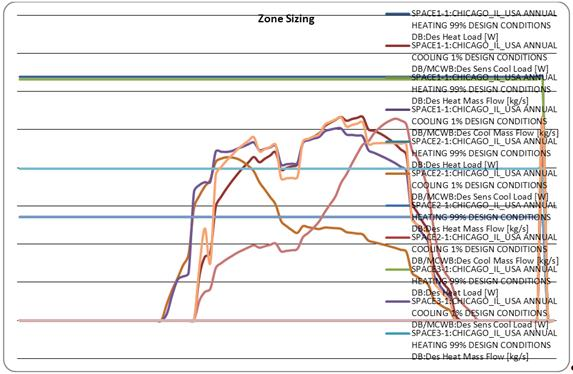
\includegraphics[width=0.9\textwidth, height=0.9\textheight, keepaspectratio=true]{media/image018.jpg}
\caption{Zone Sizing from epluszsz.csv \protect \label{fig:zone-sizing-from-epluszsz.csv}}
\end{figure}
